\documentclass{article}
%===================================== Package Info ================================%

\usepackage{graphicx}
\usepackage{xcolor}
\usepackage{cite}
\usepackage{hyperref}
\usepackage{authblk}
\graphicspath{ {.} }
\title{Stationary and non-stationary timeseries data}
\author{Alireza Miraliakbar}
\affil{School of Chemical Engineering, Oklahoma State University, Stillwater, OK, 74078}
\date{Spring 2024}
\bibliographystyle{abbrv}

\begin{document}
\maketitle
The concept of stationary and non-stationary is important about each process variable 
timeseries data, as it directly influences the choice of data analysis method. The concept 
was a bit vague for me when encountered, so I decided to write this document for better understanding
of it. 
Let's first take a look at definitions:
\newline 
\\
\textbf{Definition 1:} a timeseries is said to be \textit{stationary} if the statistical 
properties of it remain constant as new samples are gathered.
\\

Figure \ref{fig:sine-wave} shows an example of a statinary datastream. 
\begin{figure}[h]
    \center 
    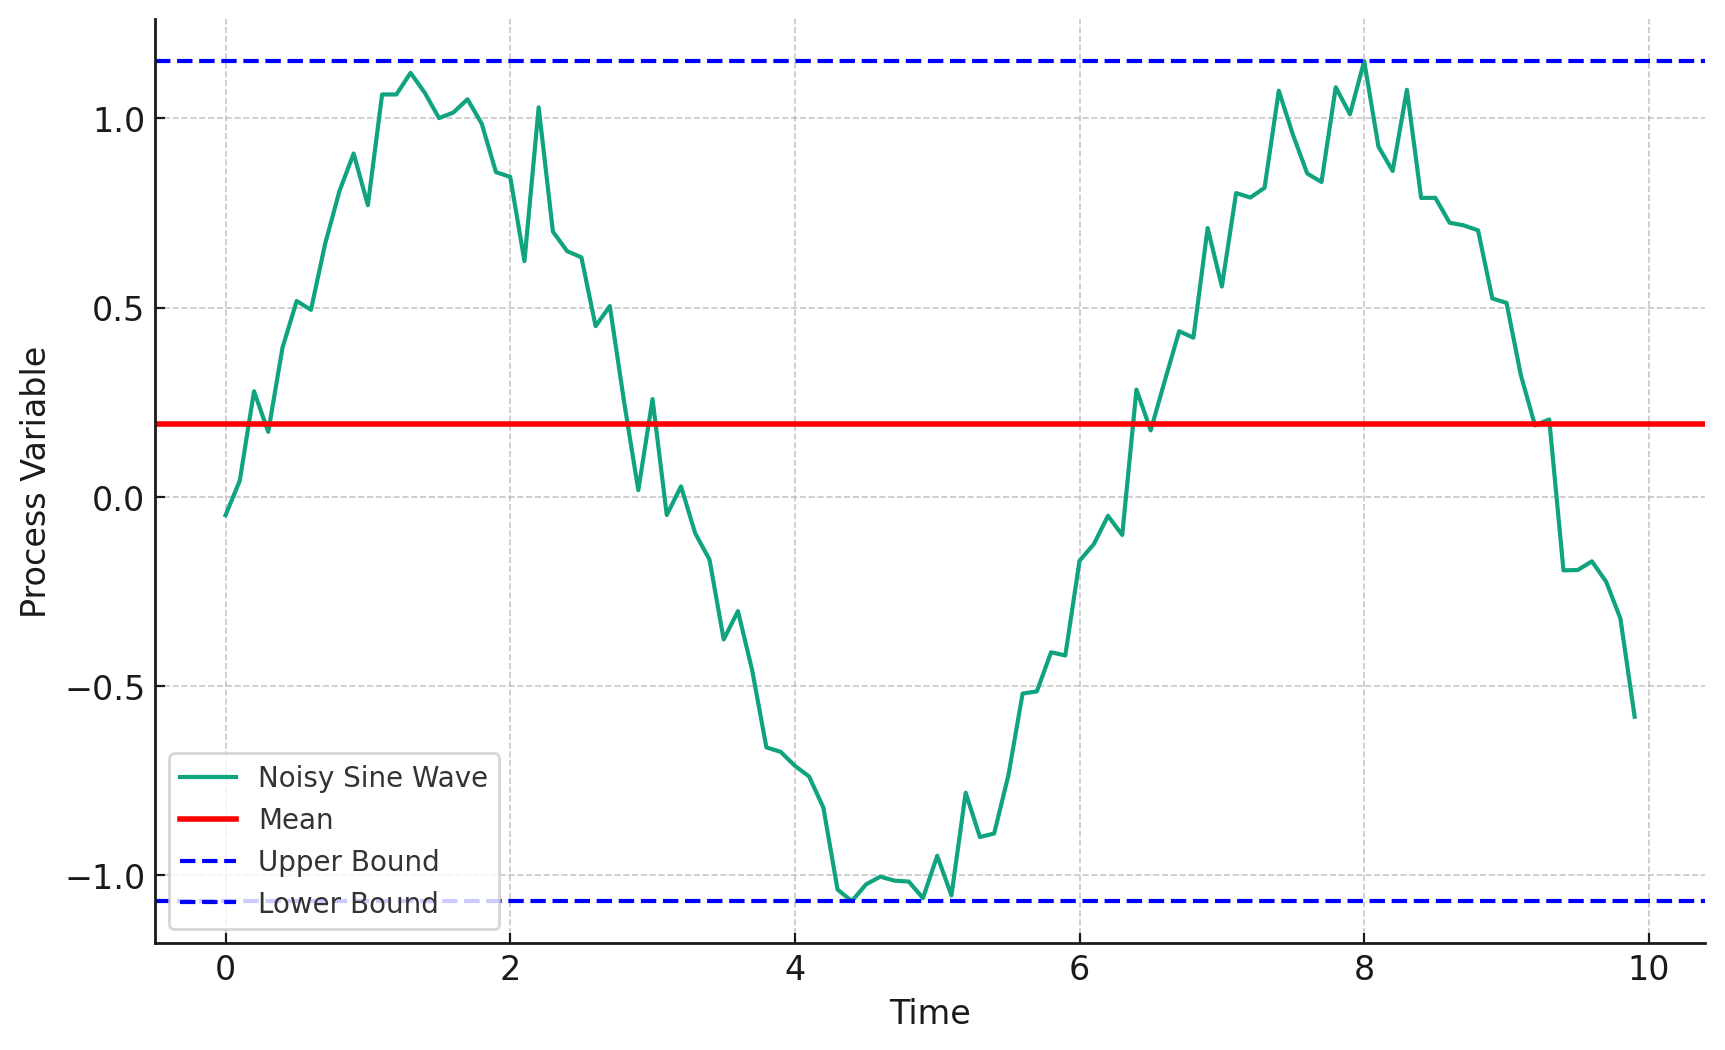
\includegraphics[width=0.8\textwidth]{stationary-wave.png}
    \caption{Stationary datastream with constant mean, variance and covariance}
    \label{fig:sine-wave}
\end{figure}

Generally, it is very ideal to have a stationary datastream in a real process. That's when the properties are
within a range, and they are assumed to be constant, we say we have a \textit{quasi-stationary} datastream.
Converging and diverging patterns of data are non-stationary, since variance changes even though the mean remains
constant.
Figure \ref{fig:converge-wave} shows an example of a statinary datastream. 
\begin{figure}[h]
    \center 
    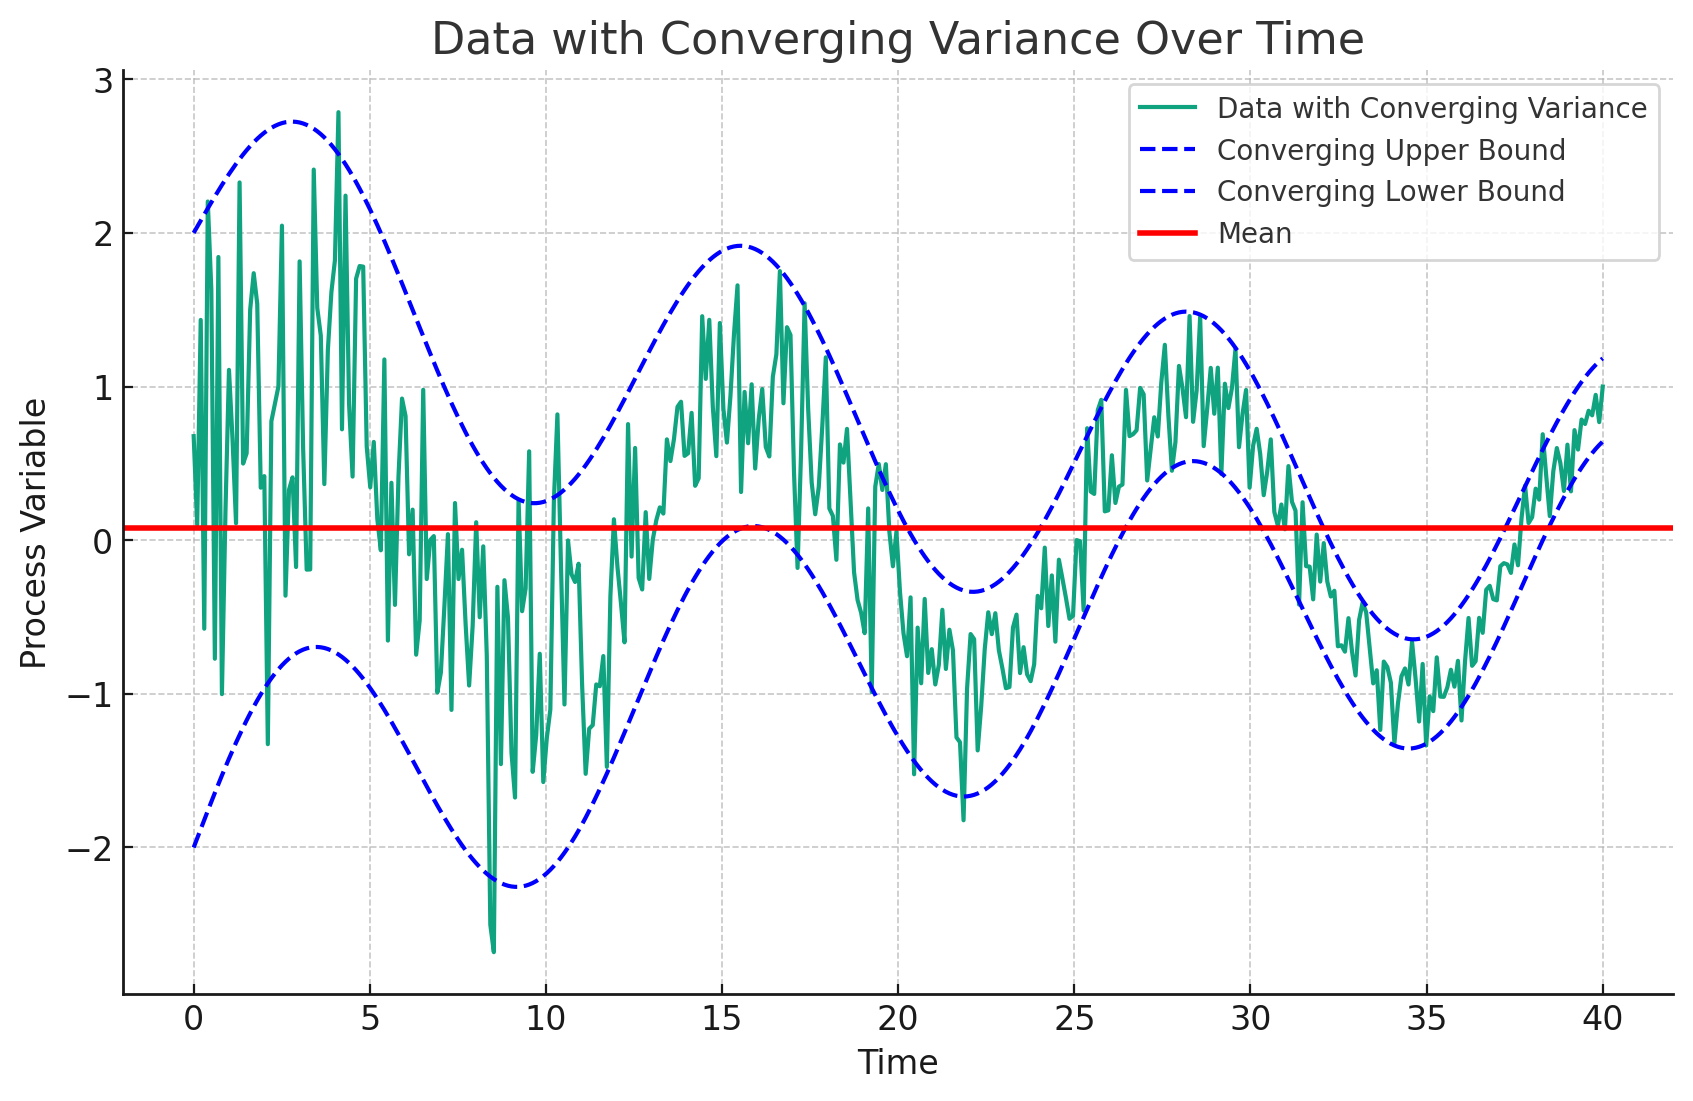
\includegraphics[width=0.8\textwidth]{convering data.png}
    \caption{Non-stationary converging datastream with constant mean and decreasing variance}
    \label{fig:converge-wave}
\end{figure}

Another case is when, mean increases(or decreases), but variance is constant.
\begin{figure}[h]
    \center 
    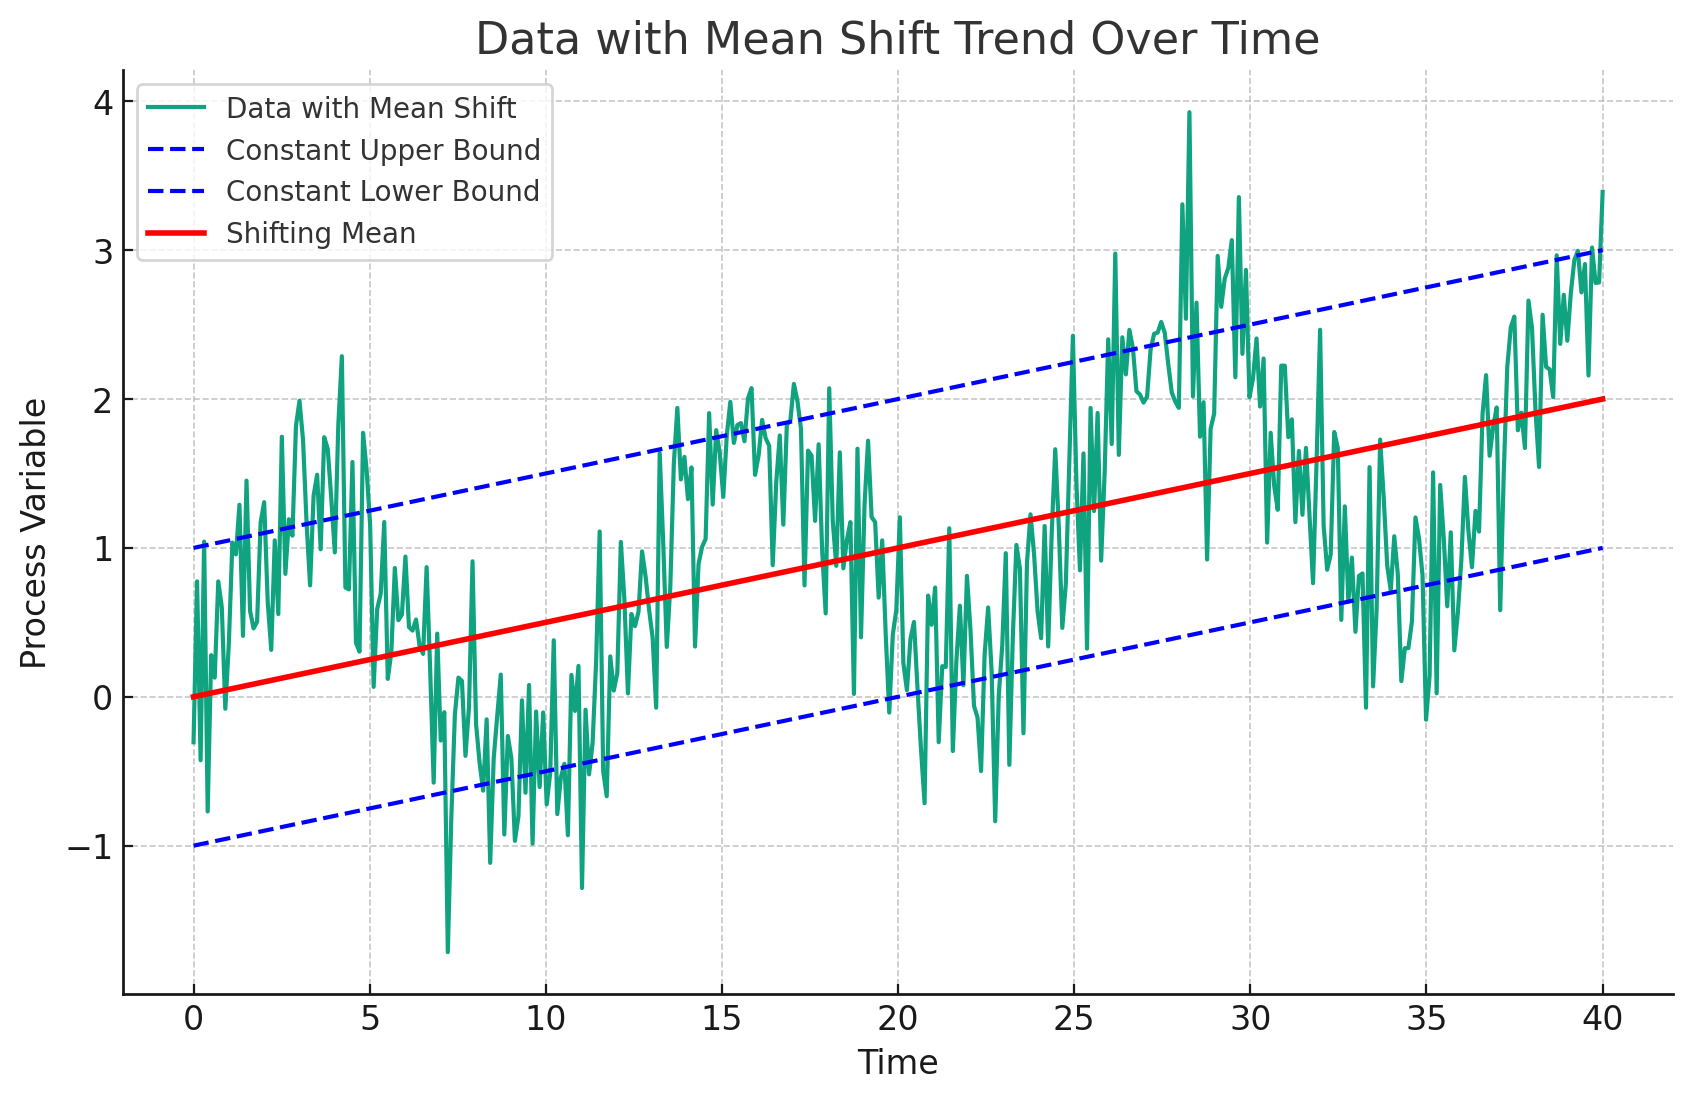
\includegraphics[width=0.685\textwidth]{meanshift.png}
    \caption{Non-stationary datastream with increase of mean and constant variance}
    \label{fig:converge-wave}
\end{figure}
\bibliography{references}
\end{document}